\documentclass{sigchi}

% Use this section to set the ACM copyright statement (e.g. for
% preprints).  Consult the conference website for the camera-ready
% copyright statement.

% Copyright
%\CopyrightYear{2016}
%\setcopyright{acmcopyright}
%\setcopyright{acmlicensed}
%\setcopyright{rightsretained}
%\setcopyright{usgov}
%\setcopyright{usgovmixed}
%\setcopyright{cagov}
%\setcopyright{cagovmixed}
% DOI
%\doi{http://dx.doi.org/10.475/123_4}
% ISBN
%\isbn{123-4567-24-567/08/06}
%Conference
%\conferenceinfo{CHI'16,}{May 07--12, 2016, San Jose, CA, USA}
%Price
%\acmPrice{\$15.00}

% Use this command to override the default ACM copyright statement
% (e.g. for preprints).  Consult the conference website for the
% camera-ready copyright statement.


% Arabic page numbers for submission.  Remove this line to eliminate
% page numbers for the camera ready copy
% \pagenumbering{arabic}

% Load basic packages
\usepackage{balance}       % to better equalize the last page
\usepackage{graphics}      % for EPS, load graphicx instead 
\usepackage[T1]{fontenc}   % for umlauts and other diaeresis
\usepackage{txfonts}
\usepackage{mathptmx}
\usepackage[pdflang={en-US},pdftex]{hyperref}
\usepackage{color}
\usepackage{booktabs}
\usepackage{textcomp}

% Some optional stuff you might like/need.
\usepackage{microtype}        % Improved Tracking and Kerning
% \usepackage[all]{hypcap}    % Fixes bug in hyperref caption zlinking
\usepackage{ccicons}          % Cite your images correctly!
% \usepackage[utf8]{inputenc} % for a UTF8 editor only

% If you want to use todo notes, marginpars etc. during creation of
% your draft document, you have to enable the "chi_draft" option for
% the document class. To do this, change the very first line to:
% "\documentclass[chi_draft]{sigchi}". You can then place todo notes
% by using the "\todo{...}"  command. Make sure to disable the draft
% option again before submitting your final document.
\usepackage{todonotes}

% Paper metadata (use plain text, for PDF inclusion and later
% re-using, if desired).  Use \emtpyauthor when submitting for review
% so you remain anonymous.
\def\plaintitle{To Clack or Not to Clack: An Investigation of Audio-Tactile cues for Typing Efficiency}
\def\plainauthor{First Author, Second Author, Third Author,
  Fourth Author, Fifth Author, Sixth Author}
\def\emptyauthor{}
\def\plainkeywords{Mechanical Keyboard; Audio-Tactile Switch; Tactile Switch; Typing Efficiency;}
\def\plaingeneralterms{Documentation, Standardization}

% llt: Define a global style for URLs, rather that the default one
\makeatletter
\def\url@leostyle{%
  \@ifundefined{selectfont}{
    \def\UrlFont{\sf}
  }{
    \def\UrlFont{\small\bf\ttfamily}
  }}
\makeatother
\urlstyle{leo}

% To make various LaTeX processors do the right thing with page size.
\def\pprw{8.5in}
\def\pprh{11in}
\special{papersize=\pprw,\pprh}
\setlength{\paperwidth}{\pprw}
\setlength{\paperheight}{\pprh}
\setlength{\pdfpagewidth}{\pprw}
\setlength{\pdfpageheight}{\pprh}

% Make sure hyperref comes last of your loaded packages, to give it a
% fighting chance of not being over-written, since its job is to
% redefine many LaTeX commands.
\definecolor{linkColor}{RGB}{6,125,233}
\hypersetup{%
  pdftitle={\plaintitle},
% Use \plainauthor for final version.
%  pdfauthor={\plainauthor},
  pdfauthor={\emptyauthor},
  pdfkeywords={\plainkeywords},
  pdfdisplaydoctitle=true, % For Accessibility
  bookmarksnumbered,
  pdfstartview={FitH},
  colorlinks,
  citecolor=black,
  filecolor=black,
  linkcolor=black,
  urlcolor=linkColor,
  breaklinks=true,
  hypertexnames=false
}

% create a shortcut to typeset table headings
% \newcommand\tabhead[1]{\small\textbf{#1}}

% End of preamble. Here it comes the document.
\begin{document}

\title{\plaintitle}

\numberofauthors{1}
\author{%
  \alignauthor{Jia Rong Wu\\
    \affaddr{PhD Candidate at Waterloo University}\\    
    \affaddr{Waterloo, Canada}\\
    \email{jr2wu@uwaterloo.ca}}\\    
}

\maketitle

\begin{abstract}
Mechanical keyboards are emerging as a popular ergonomic and effective alternative to membrane keyboards. There are a myriad of mechanical key-switches on the prosumer market, yet little research available to illuminate whether or not one switch is better than another for typing efficiency. This study aims to investigate the effect of audio cues when using mechanical key-switches. A 2 x 3 within-subject design experiment will be conducted where participants will be asked to input text of varying length. We ultimately expect this work to serve as a base for consumers and companies looking to boost efficiency when interacting with computers through keyboards.
\end{abstract}

\category{H.5.2}{User Interfaces} {Ergonomics; Input devices and strategies;}

\keywords{\plainkeywords}

\section{Introduction}
Mechanical keyboards have a long and rich history dating back to the 1970s when Alps Electronics and International Business Machines built keyboards such as the Alps SCB1A163 and IBM 3276 (add citation here). These early models were mechanical in the sense that each key switch was an independent functional unit. Cherry GmbH took the concept further with their key switch design formalized in the U.S. Patent 4,467,160. This would go on to be the blueprint for the design of the modern mechanical switch \cite{switch:cherry}. \\

There are virtually unlimited configurations for keyboards, including physical layouts, software layouts, keycap shapes and key switch choice. In a mechanical keyboard, each key switch, hereafter referred to as a switch, is comprised of an individual housing, spring and stem along with optional tactile features. Tactile features are used to indicate to users when the switch has actuated or registered a stroke. These features can be located at differing distances of switch depression along with different levels of force depending on the tactile mechanism. In some switch variants, audio cues in the form of click bars may be used to provide additional audio-tactile feedback as opposed to simple tactile feedback. \\

In this paper we describe experiments that will investigate typing efficiency of users using tactile and audio-tactile switches. The questions we aim to address are as follows: Do audio-tactile cues provide benefits to users in the form of increased typing speed? Do audio-tactile cues reduce the typing error of users? Do audio-tactile cues allow users to input characters with more precision? Thus our null hypotheses become; H0: There is no difference in typing speed between tactile and audio-tactile switches. H1: There is no difference in error for text entry between tactile and audio-tactile switches. \\

\section{Related Work}
Research on mechanical switches is not a novel field. Prior work in the field has primarily been related to collecting electromyogram data of finger and forearm muscles for switches that actuate at different weights \cite{martin:1996, rempel:1997, radwin:1999, gerard:1999}. Martin et al. investigated the relationship between finger force exertion and keyboard reaction forces. They used switches with a 48g actuation weight and measured the maximal voluntary contraction of each finger. In their discussion, they theorized that providing feedback to keyboard users may allow for a reduction in force required to actuate switches at high typing speeds \cite{martin:1996}. Gerard et al. examined how the actuation weight of a switch affects user discomfort and typing force. While they only examined the tactile aspect of switches, they discovered that keyboards with better feedback characteristics allowed users to type with less discomfort and less force \cite{gerard:1999}. \\

Studies have been conducted which measure the typing efficiency of keyboards with variable switch travel distances. Hughes et al. compared typing efficiency across three separate keyboards with identical actuation forces, but differing travel distances of 2.0mm, 2.5mm and 4.0mm \cite{hughes:2011}. They determined that there was no statistically significant difference between typing speed or accuracy between these three conditions. Comparisons have also been drawn between the typing speed of membrane based switches and mechanical switches \cite{pham:2015}. Pham et al. investigated if there was a difference in typing performance between membrane based keyboards and mechanical based keyboards. Their results indicated no significant difference between those types of keyboards.\\

Providing audio feedback for software based keyboards has been shown to decrease the time required to enter phrases in mobile and tablet devices \cite{hoggan:2010, hoggan:2009}. Ma et al. investigated the effect of haptic and audio feedback on both typing speed and typing errors \cite{ma:2015}. Their study design utilized a flat immobile keyboard, and a haptic engine design which could deliver tactile feedback in the form of vibrations to a user's finger, or to the entire keyboard. The authors were able to demonstrate that localized haptic feedback on a flat keyboard could improve typing performance by reducing errors and increasing typing speed. To the best of the authors' knowledge, there is no study at the time of this work that investigates the effect of switch based audio tactile cues on typing efficiency for hardware based keyboards. \\

\section{Implementation}
A minimum of twelve participants will be recruited for this study. Initially, the participants will be asked to answer a short questionnaire collecting metadata about the participants. The data being collected will include information such as self-reported typing ability, English familiarity, QWERTY layout familiarity, and mechanical keyboard familiarity. This data will be used to control for and potentially explain outliers in the experimental data. The participants will then be asked to participate in a typing exercise in which they enter phrases onto WebTEM. \\

The Massdrop CTRL Mechanical Keyboard with hot-swap switch sockets will be used as the keyboard base for this experiment \cite{ctrl:keyboard}. It is an 87-switch keyboard with switches organized in a QUERTY key layout following the ANSI physical layout. The key caps provided will be DSA profile as indicated in \ref{fig:oem_cherry_dsa}. While common profiles for most keyboards are OEM or CHERRY with the flat keycap design, DSA profile keycaps have a slightly scooped design. Switches used in this experiment will be Kailh Box Burnt Oranges and Kailh Box Navys. Both switches are tactile, have a 3.6mm travel, and have an actuation force of 60g \cite{switch:navy, switch:orange}. Box Navy switches are audio-tactile switches containing a additional click bar. This bar does not affect the actuation force and provides an audio cue upon switch actuation. \\

\begin{figure}
\centering
  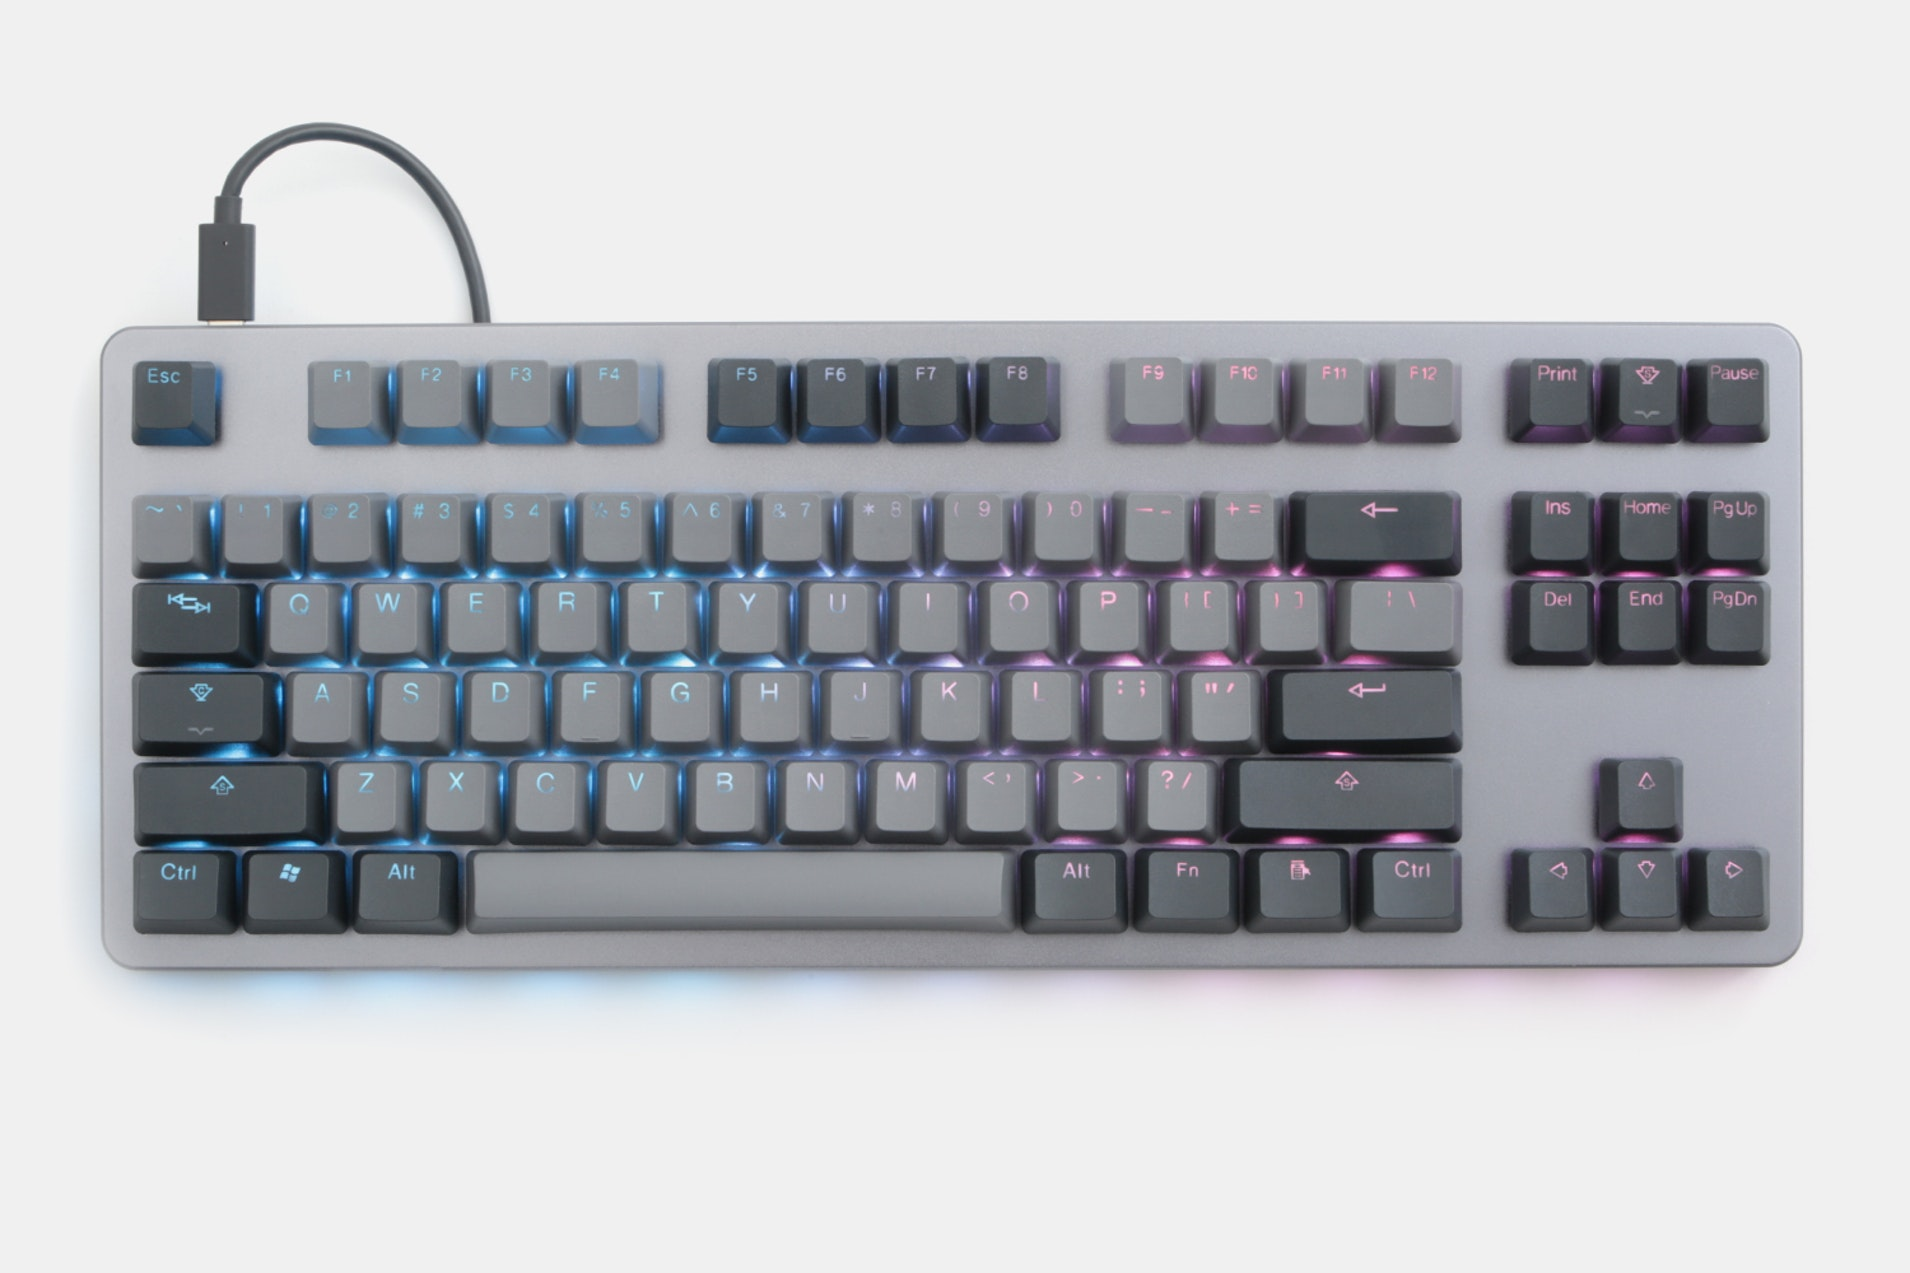
\includegraphics[width=0.9\columnwidth]{figures/ctrl_top_view}
  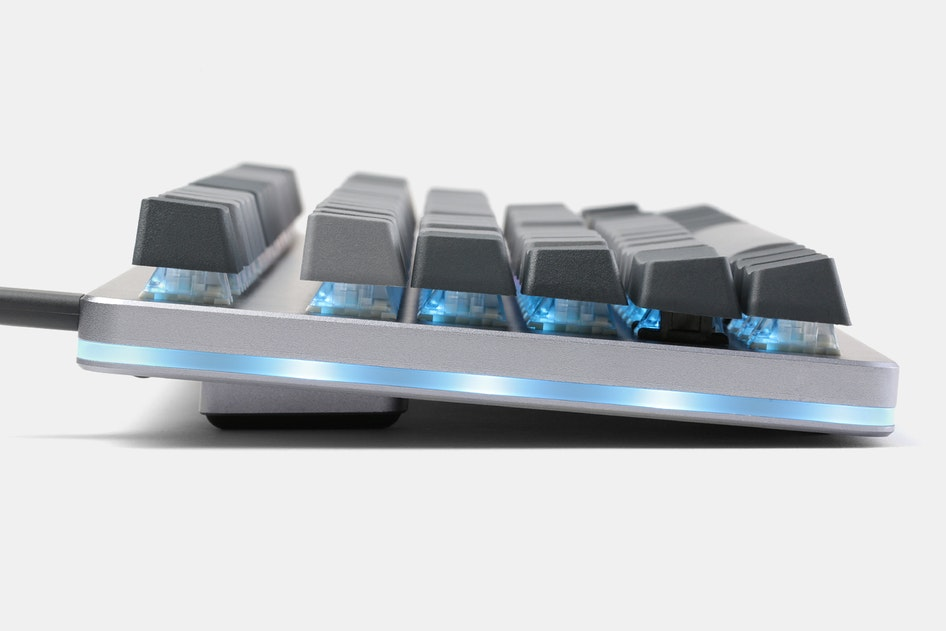
\includegraphics[width=0.9\columnwidth]{figures/ctrl_side_view}
  \caption{The Massdrop CTRL Mechanical Keyboard. Pictured with OEM Keycaps. }~\label{fig:ctrl_top_view}
\end{figure}
\begin{figure}
\centering
  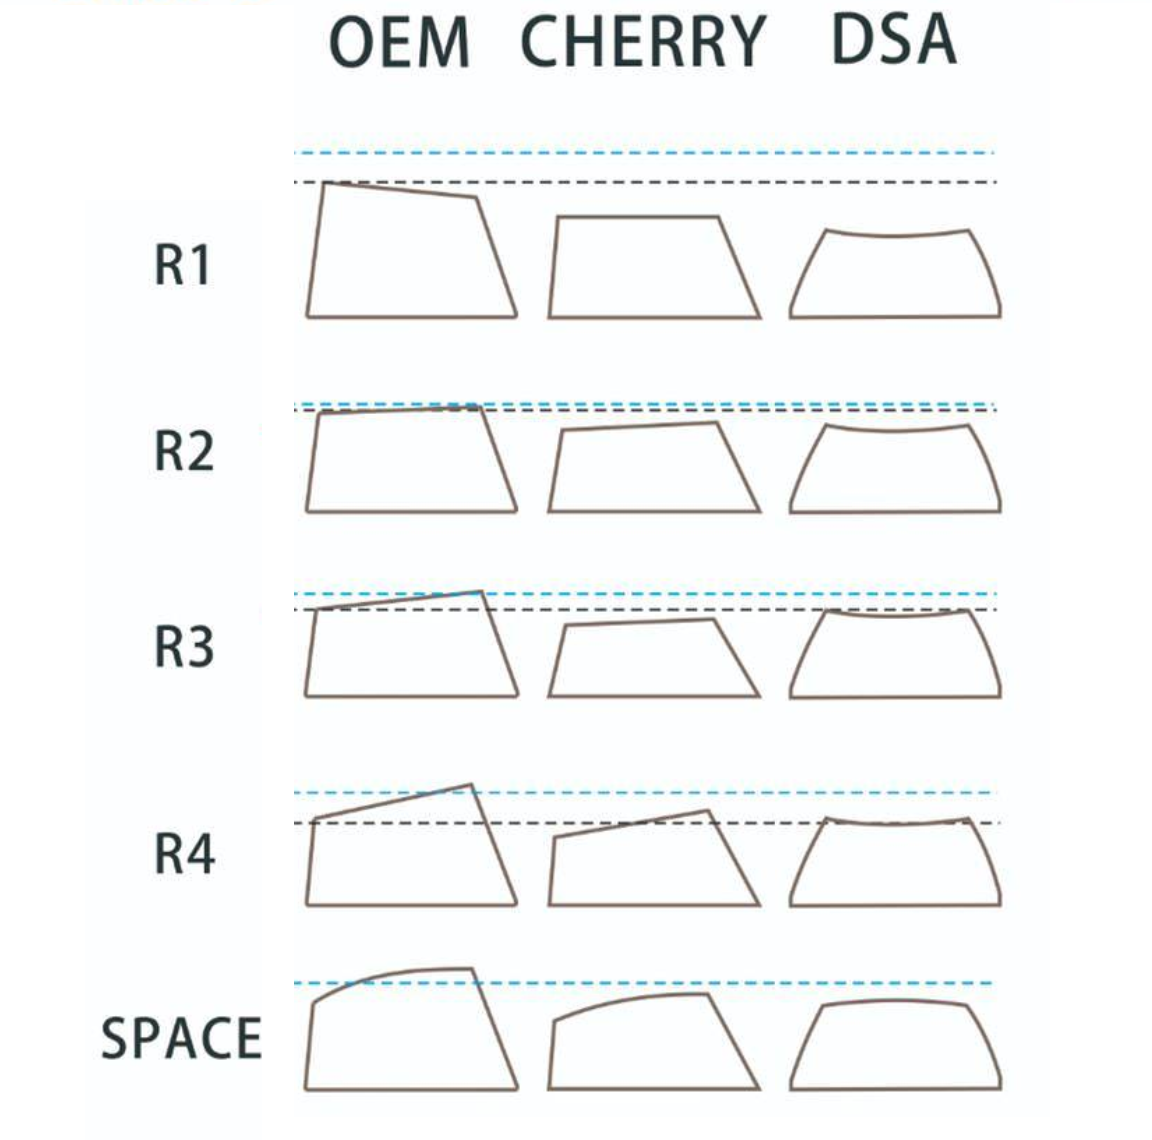
\includegraphics[width=0.9\columnwidth]{figures/oem_cherry_dsa}
  \caption{Common Keycap Profiles}~\label{fig:oem_cherry_dsa}
\end{figure}

Prior to the experiment, participants will be given two minutes to familiarize themselves with the keyboard and adjust ergonomic settings such as chair and keyboard height. In order to test out H0 and H1, participants will be asked to type out sets of short, medium, and long phrases with varying lengths on the Massdrop CTRL with either the Burnt Orange or Navy switches inserted. This implies there will be two independent data collection sessions per participant due to the need to swap out the switches. Half the participants will begin the experiment with tactile switches, and half the participants will begin with audio-tactile switches. \\

WebTEM, a web application for recording text entry metrics will be used to log information about phrases that users will input \cite{arif:2016}. Subsequent statistical data analysis will be conducted using R and Python. Participants will be instructed to type the phrases as quickly as possible and their error rates will be measured. There will be a 1 minute break provided between each block. The experiment will use a 2 x 3 within-subject design for the factors: (tactile or audio\_tactile) and block. Within each set of phrases, the order in which they appear to the participants will be randomized.\\

After the exercise, participants will be asked to provide a brief description of their experience with the keyboard. Topics asked will include whether or not they preferred one keyboard to the other, their comfort level with the keyboard and overall how usable the keyboard was. \\

\section{Results}


\section{Discussion}
H0: There is no difference in typing speed between tactile and audio-tactile switches. 


H1: There is no difference in error for text entry between tactile and audio-tactile switches.

\subsection{Limitations}
Mention if participants were used to mechanical keyboards. The time allocated for participants to familiarize themselves with the keyboard may not have been enough. 

Average decibel readings for the room ranged from anywhere between 55Db to 62Db. While unlikely, this extraneous noise might have negated the benefits of having an audio feedback.

Keys were heavier than participants expected or were used to.

Users mentioned the key travel distance was large, and would have benefited from a elevated wrist rest. 

No range finders for F and J keys. 

Spelling was American as opposed to Canadian. 

Different location(s) for conducting experiment.




\section{Future Work}

% BALANCE COLUMNS
\balance{}

% REFERENCES FORMAT
% References must be the same font size as other body text.
\bibliographystyle{SIGCHI-Reference-Format}
\bibliography{sample}

\end{document}

%%% Local Variables:
%%% mode: latex
%%% TeX-master: t
%%% End:
